%%PREAMBLE %%%%%%%%%%%%%%%%%%%%%%%%%%%%
\documentclass[10pt, a4paper]{article}% size of txt = 10pt
\usepackage[top= 2cm,
			bottom = 2cm,
			left = 1.7cm,
			right = 1.7cm,
			footskip = 0.5cm,
			headsep = 0cm,
			headheight = 0cm
					]{geometry}
\usepackage{amsmath} % math packages
\usepackage{amsfonts}% math packages
\usepackage{amssymb} % math packages
\usepackage{graphicx} %package for including graphics
\usepackage{array}
\usepackage[thinlines]{easytable}
\usepackage{float}
\usepackage[section]{placeins}
\usepackage[hidelinks]{hyperref}
\usepackage[shortlabels]{enumitem}
\usepackage{svg}
\usepackage{bigstrut}
\usepackage{wrapfig,lipsum,booktabs}
\usepackage{subcaption}
\usepackage{xfrac}
\usepackage{pdfpages}
\usepackage{listings}
\usepackage{xcolor}


\usepackage{listings}
\usepackage{color} %red, green, blue, yellow, cyan, magenta, black, white
\definecolor{mygreen}{RGB}{28,172,0} % color values Red, Green, Blue
\definecolor{mylilas}{RGB}{170,55,241}

\definecolor{codegreen}{rgb}{0,0.6,0}
\definecolor{codegray}{rgb}{0.5,0.5,0.5}
\definecolor{codepurple}{rgb}{0.58,0,0.82}
\definecolor{backcolour}{rgb}{1,1,1}

\lstdefinestyle{mystyle}{
    backgroundcolor=\color{backcolour},   
    commentstyle=\color{codegreen},
    keywordstyle=\color{magenta},
    numberstyle=\tiny\color{codegray},
    stringstyle=\color{codepurple},
    basicstyle=\ttfamily\footnotesize,
    breakatwhitespace=false,         
    breaklines=true,                 
    captionpos=b,                    
    keepspaces=true,                 
    numbers=left,                    
    numbersep=5pt,                  
    showspaces=false,                
    showstringspaces=false,
    showtabs=false,                  
    tabsize=2
}
\lstset{style=mystyle}


%date format
\def\mydate{\leavevmode\hbox{\twodigits\day.\twodigits\month.\the\year}}
\def\twodigits#1{\ifnum#1<10 0\fi\the#1}

\usepackage{indentfirst}
\setlength{\parindent}{1cm}

\makeatletter
\newcommand{\thickhline}{%
    \noalign {\ifnum 0=`}\fi \hrule height 2pt
    \futurelet \reserved@a \@xhline
}
\newcolumntype{"}{@{\hskip\tabcolsep\vrule width 2pt\hskip\tabcolsep}}
\makeatother
\newcolumntype{?}{!{\vrule width 2pt}}
%%DOC ENVIROMENT%%%%%%%%%%%%%%%%%%%%%%%
\begin{document}
%Title 
\begin{flushleft}%% left justification
	\textbf{\Large{MKC-IKS: Úkol č. 1}}\hfill Filip Paul\\
	\large{CORDIC \hfill\mydate}
\end{flushleft}


	\section{\Large Úkol 1:}
		Uvažujte algoritmus CORDIC v módu vektorové rotace. Kolik iterací je třeba pro otočení počátečního vektoru [0.5  0.5]
		o -40° s chybou menší než 0,5°? Průběh jednotlivých iterací (zejména aktuální úhel) popište numericky a doplňte přehledným obrázkem. (2 body)\\
		Úkol byl řešen pomocí MATLABU, příslušné scripty si můžete zobrazit v mém GITHUB repozitáři 
		\href{https://github.com/FilipPaul/ctvrtak_letni_semestr/blob/main/MKC_REM/ukol_1_CORDIC/README.md}{\color{blue} zde}.
	\begin{figure}[ht!]
		\centering
		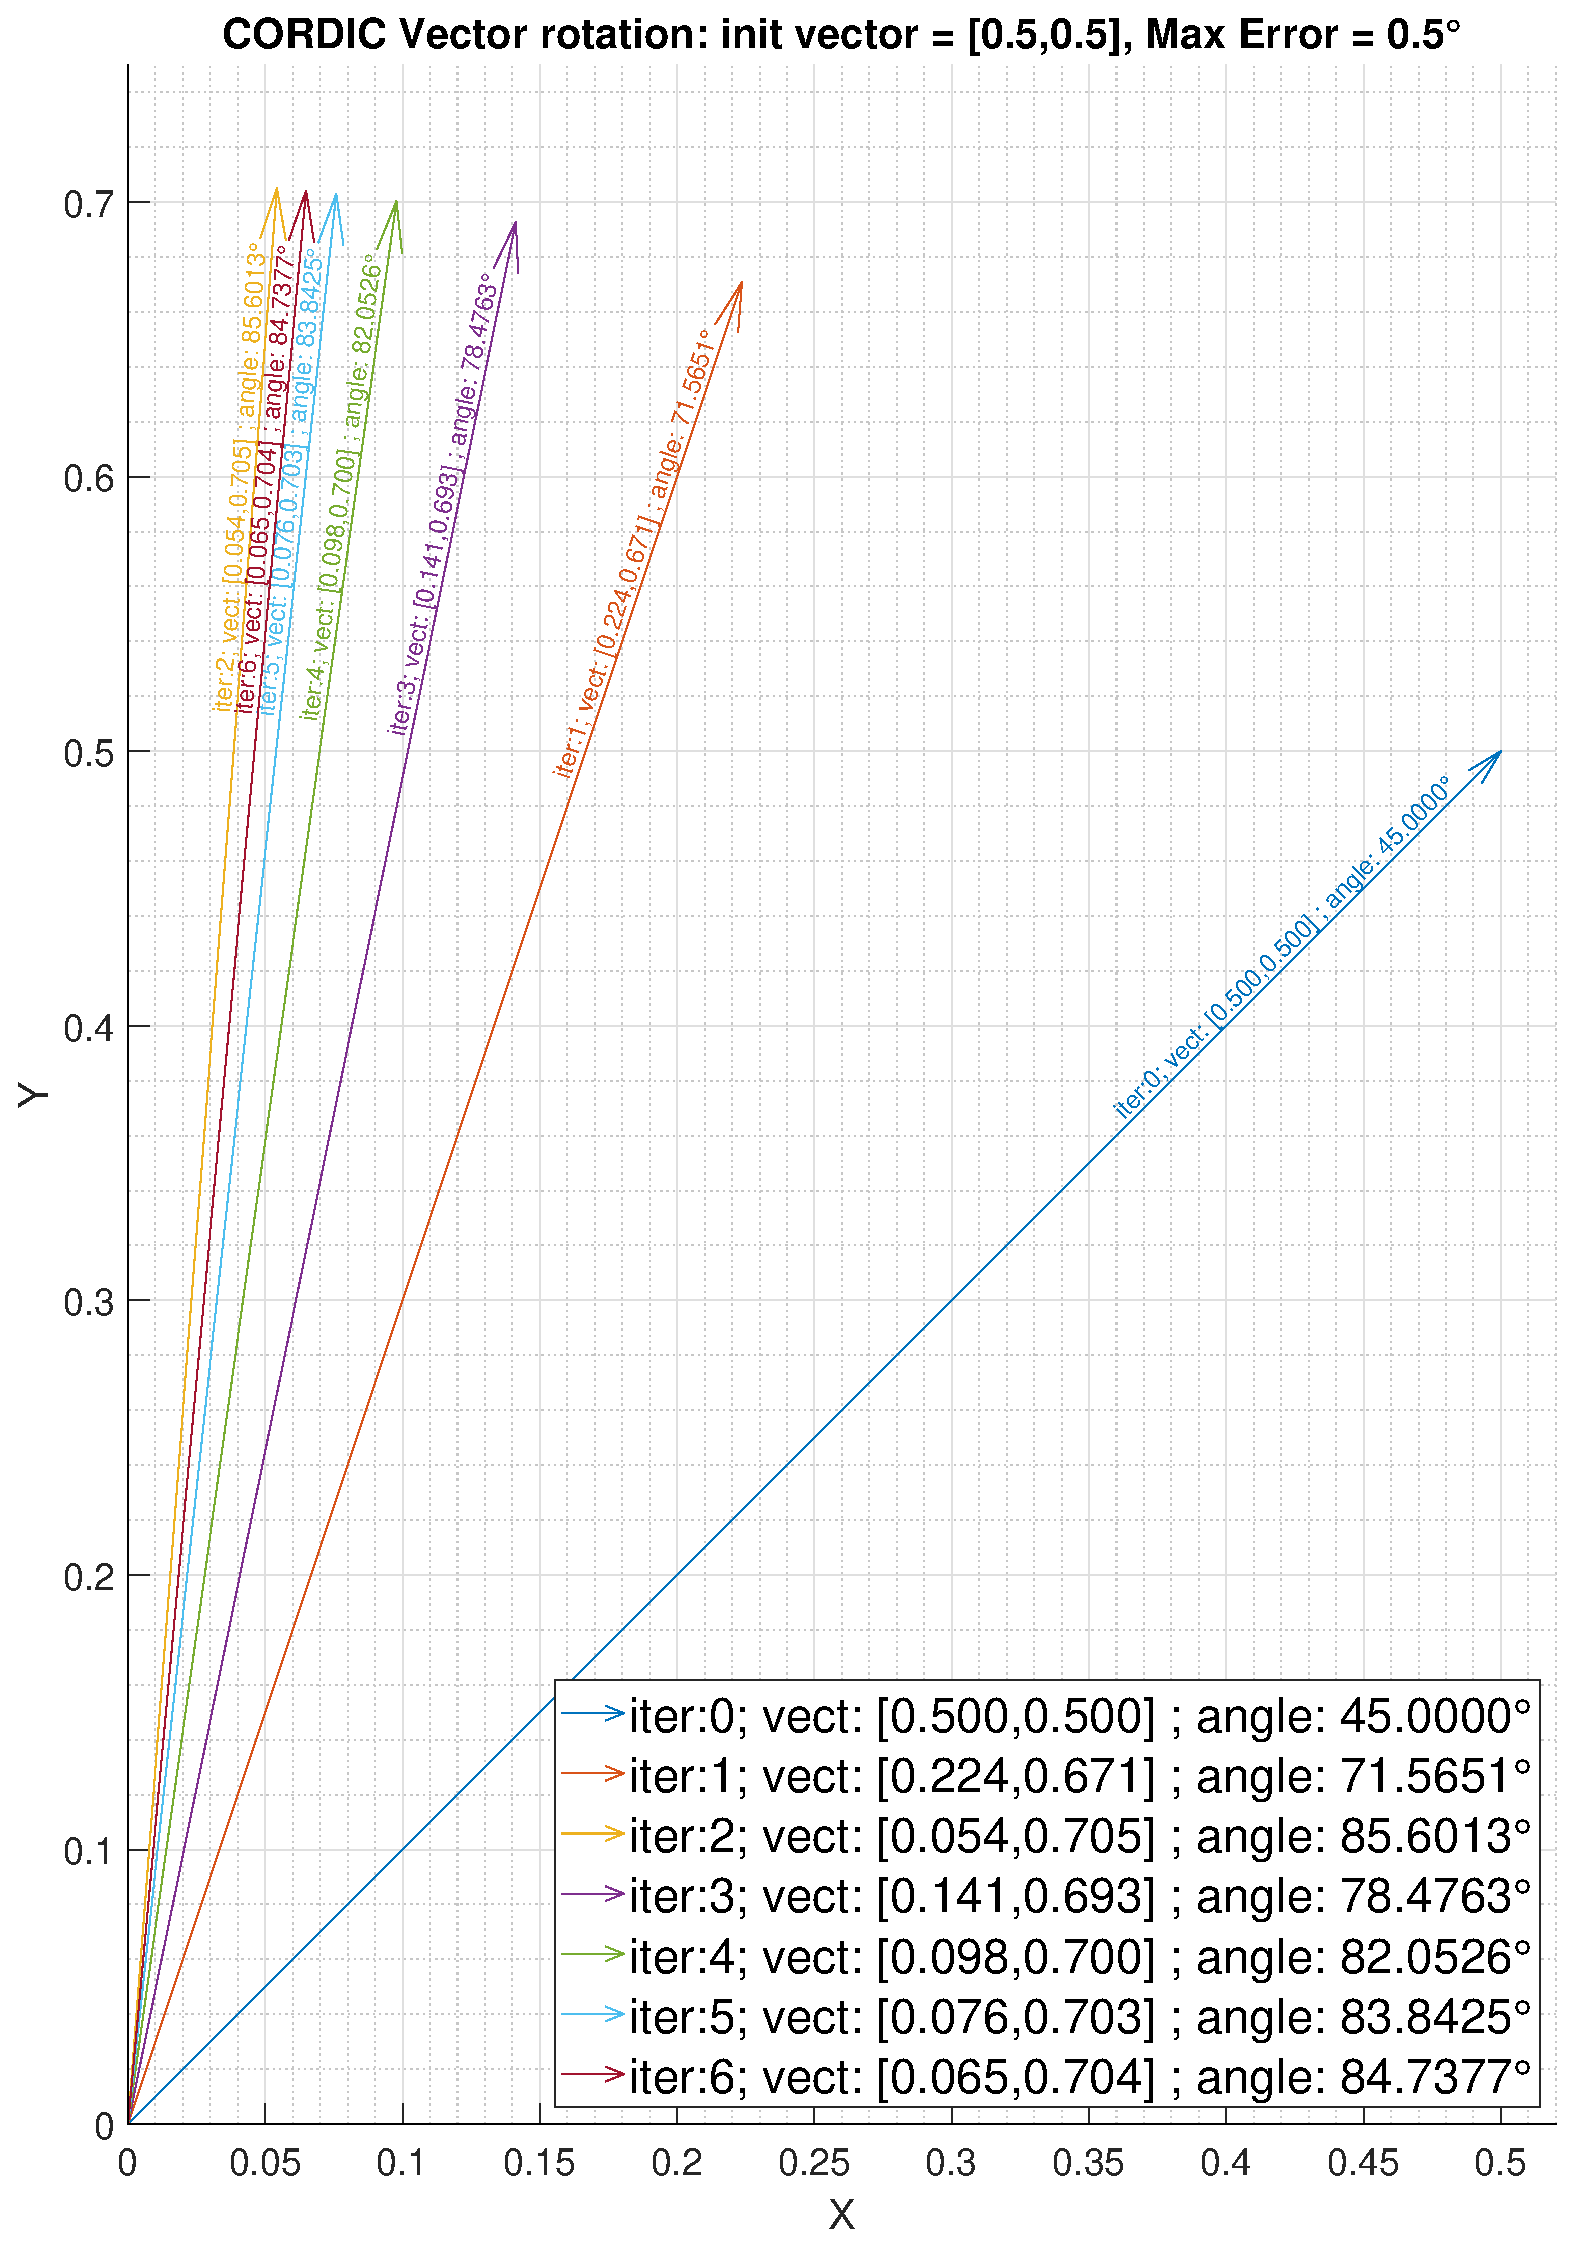
\includegraphics[height = 0.80\textheight]{CORDIC_vect_rot.eps}
		
	\end{figure}
	\clearpage
	\section{\Large Úkol 2:}
	Uvažujte algoritmus CORDIC v módu vektorové translace. Vstupní vektor je [0.5  0.25].
	Průběh jednotlivých iterací zapište numericky a doplňte vhodným obrázkem. (2 body)\\
	Obdobně jako v prvním úkolu, byl problém řešem pomocí MATLABU. V tomto případě,
	stačila pouze jedna iterace pro dosažení úhlu 0°.
	\begin{figure}[ht!]
		\centering
		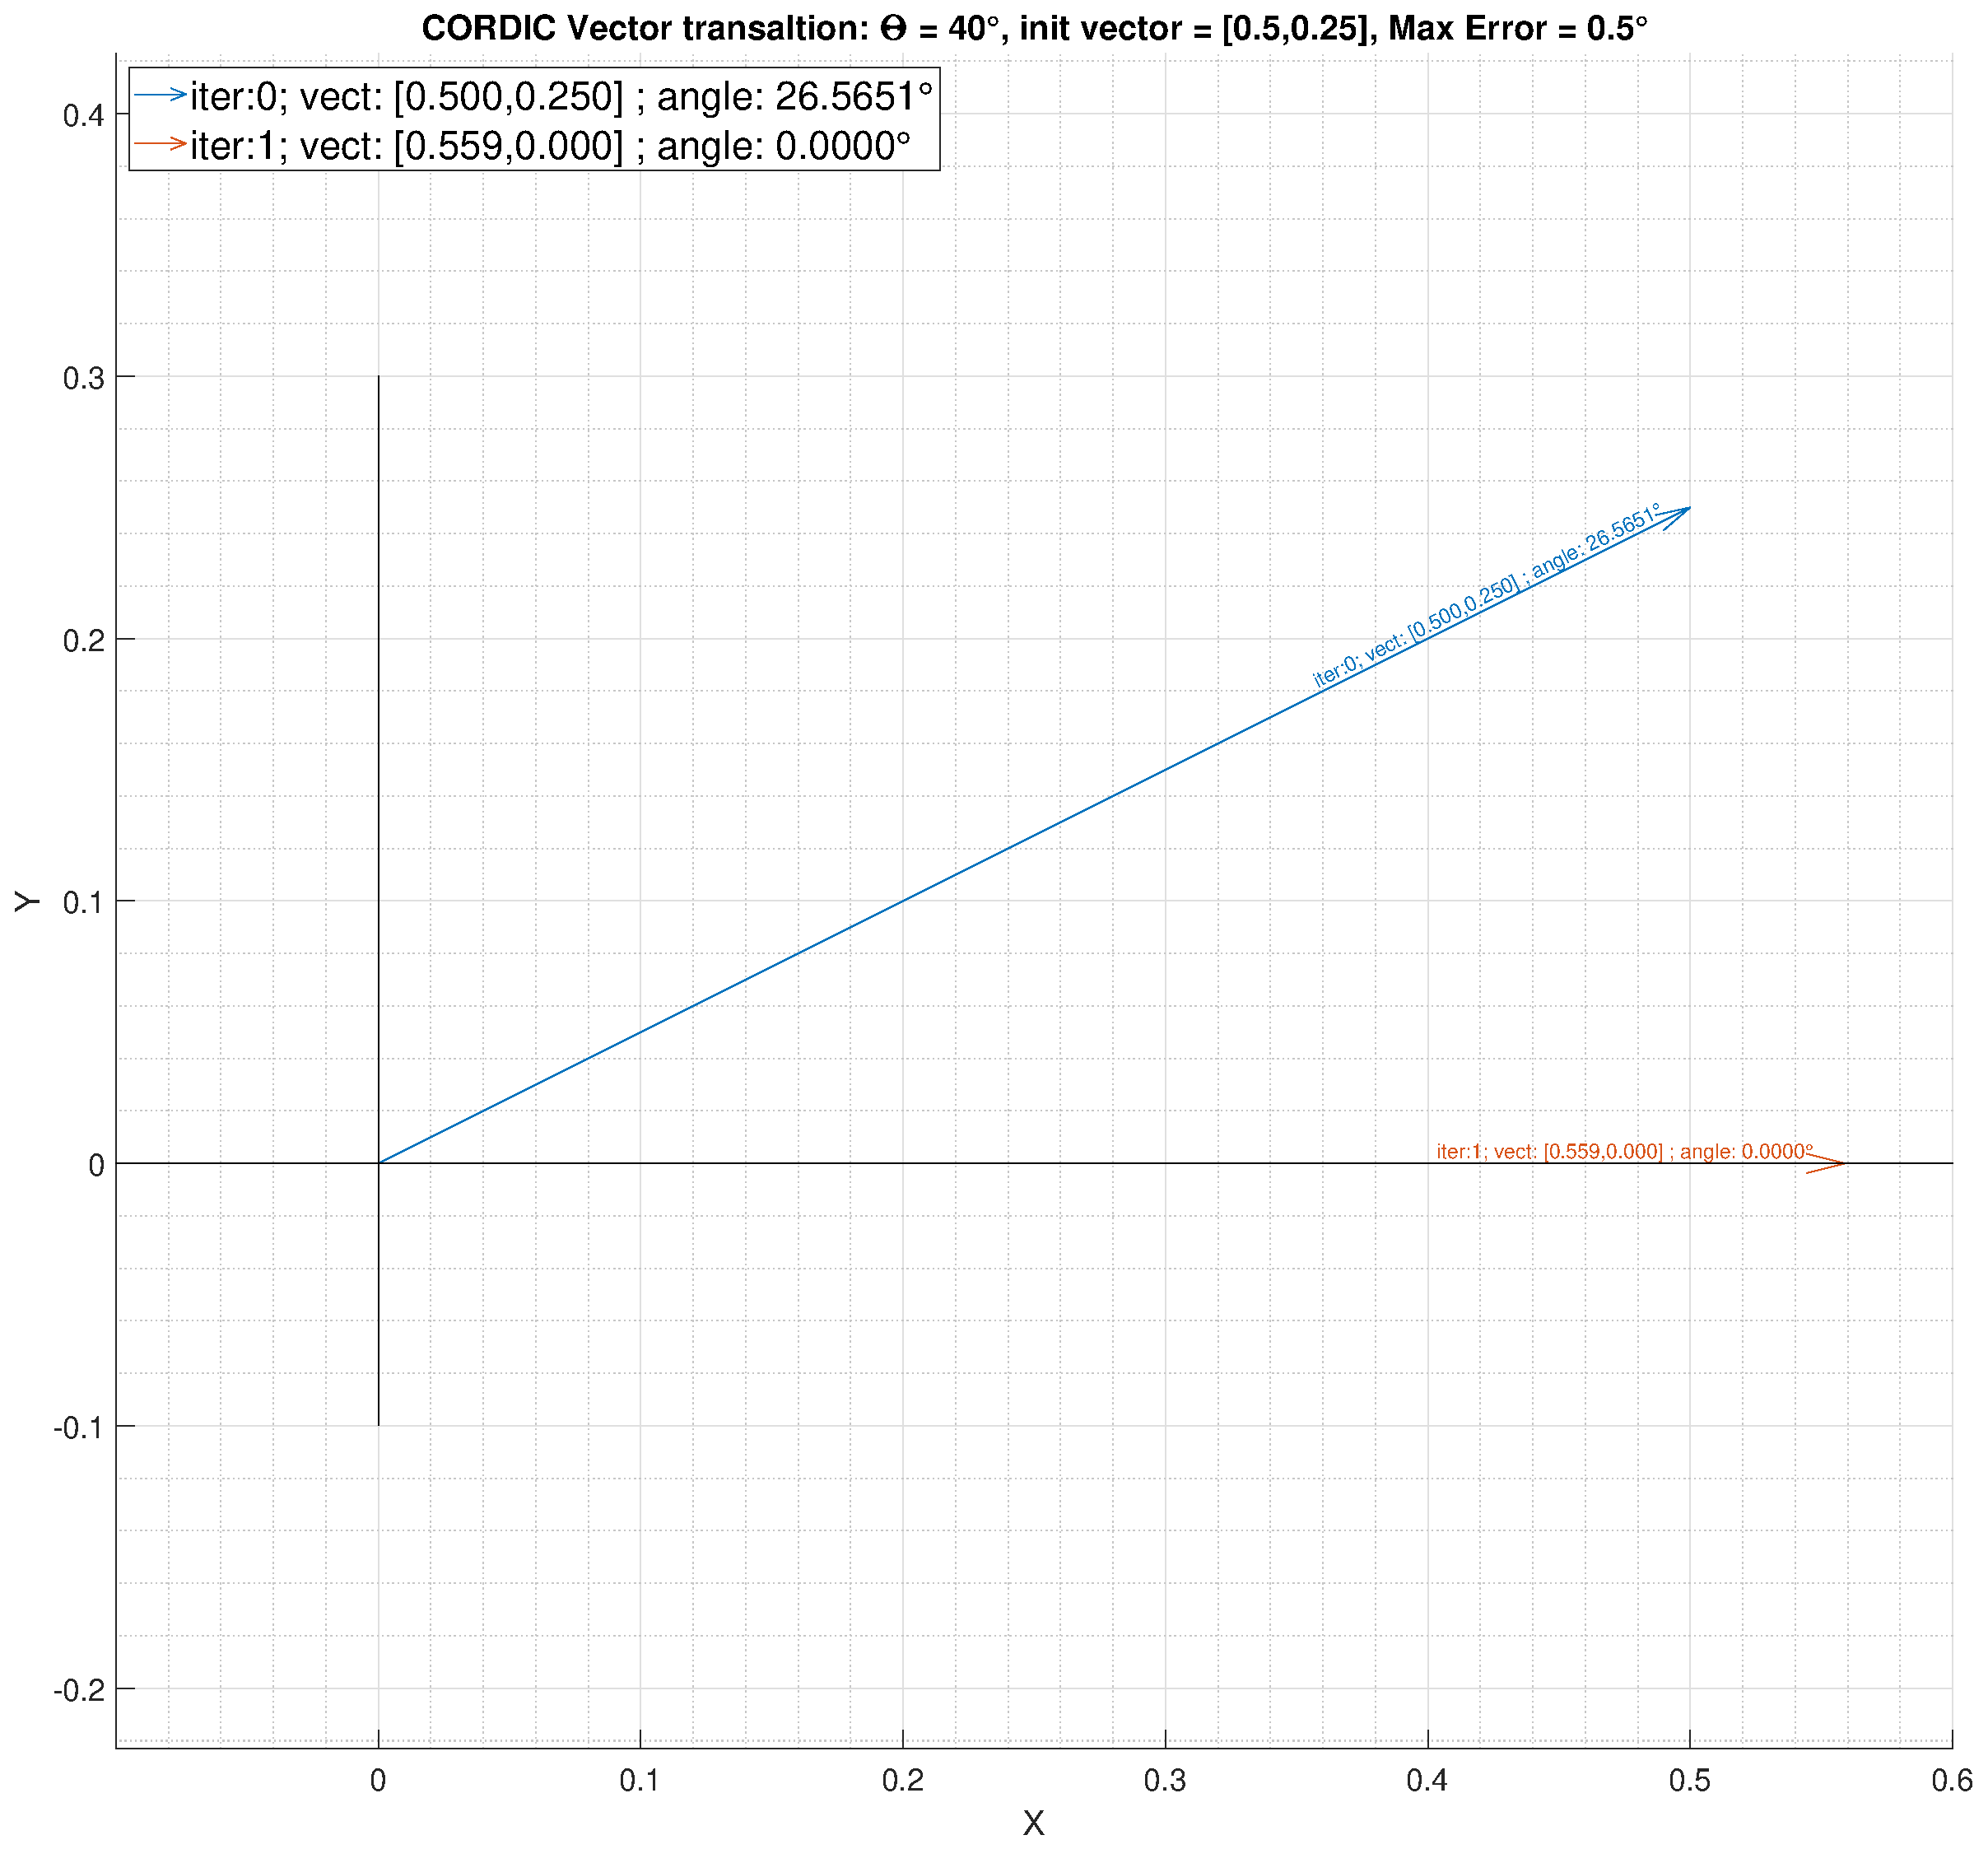
\includegraphics[width = 1\textwidth]{CORDIC_vect_trans.eps}
		
	\end{figure}
	
	\section*{\Large Vypracování:}
	placeholder

	\section{\Large Zadání:}
	Jakým způsobem je třeba algoritmus CORDIC upravit, aby pracoval ve všech kvadrantech? (2 body).
	Inspirací vám může být například následující obrázek:

	\section*{\Large Vypracování:}
	placeholder

\end{document}

%\[f(x)= (x+2)^2 - \frac{9\cdot 2\pi}{26}\] %%mathematic equatation in display style mode
%%optional:
%	\begin{align} %%this alignes all charakters after & if *is removed equations will be numbered
%	\hspace{5cm}  
%		 x &= a_2 x^2 +_1 x + a_0 \\
% 		x &=x^2 \nonumber		%no number will not add number to eq
%	\end{align}